\documentclass[../Languages.tex]{subfiles}

\begin{document}
\usec{Rust}\label{sec:rust}

\cd{Rust} is a systems programming languages sponsored by Mozilla Research,
which describes it as a ``safe, concurrent, practice language'', supporting
functional and imperative-procedural paradigm. \cd{Rust} is syntactically
similar to \cd{C++}, but its designers intended it to provide better memory
safety whilst maintaining performance.

\cd{Rust} is an open source programming language. Its designers have refined
the language through the experiences of writing the Servo web browser layout
engine and the \cd{Rust} compiler. A large portion of current commits to the
project are from community members.

\cd{Rust} won first place for ``most loved programming language'' in Stack
Overflow Developer Survey in 2016 and 2017; it is referenced in The Book of
Mozilla as ``oxidized metal''.

\subsection{Influence}\label{sub:influence}

\begin{Figure}
  \centering
  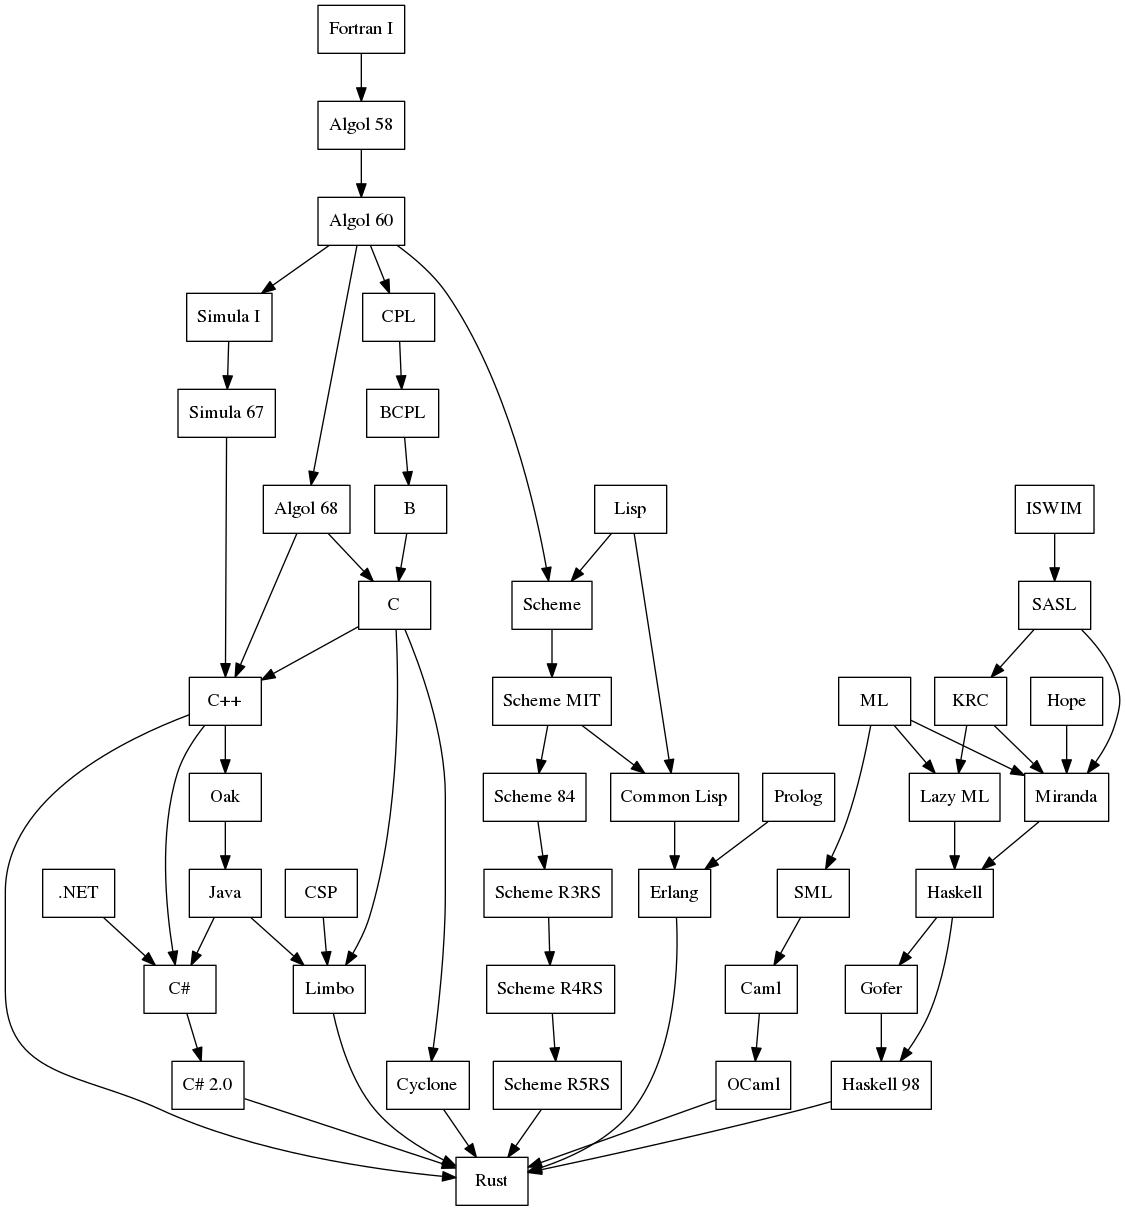
\includegraphics[height=0.5\textheight]{rust}
  \captionof{figure}{Inheritance diagram for \cd{Rust}.}
\end{Figure}

\newpage
\end{document}
